%%%%%%%% Klassen-Optionen
\documentclass[12pt,a4paper]{scrartcl}

%%%%%%%% PAKETE: unverzichtbare Pakete mit Einstellungen
\usepackage[left=2.5cm, right=2cm, top=3cm, bottom=3cm, a4paper]{geometry} %Seitenrände
\usepackage[applemac]{inputenc} % utf8-Kodierung und direkte Eingabe von Sonderzeichen
\usepackage{fixltx2e} % Verbessert einige Kernkompetenzen von LaTeX2e

%%%%%%%% PAKETE: AMS-Pakete
\usepackage{amsmath} % Mathe-Erweiterung
\usepackage{amsfonts} % Schrift-Erweiterung
\usepackage{amssymb} % Sonderzeichen-Erweiterung

%%%%%%%% PAKETE: Sonstiges
\usepackage[colorlinks, citecolor=black, filecolor=black, linkcolor=black, urlcolor=black]{hyperref} % Links
\usepackage{wrapfig} % ausgeklügekte Floatumgebung
\usepackage{float} % normale Floatumgebung
\restylefloat{figure} % ermöglicht die Verwendung von "H" (ist noch stärker als "h!")
\usepackage[small,it,singlelinecheck=false]{caption} % Bildunterschriften formatieren
\usepackage{multirow} % ermöglich Verbinden von Tabellenzeilen
\usepackage{multicol} % ermöglicht Spalten
\usepackage{fancyhdr} % ermöglicht Kopf- und Fußzeilen
\usepackage{graphicx} % Einbinden von Bildern möglich
\usepackage{units} % Einheiten
\usepackage{subcaption}

%%%%%%%% DEFINITIONEN: Titelseite
\author{April Cooper, Patrick Kreissl und Sebastian Weber}
\title{Worksheet 1: Quantum mechanical approaches:
H�ckel approximation and DFT methods}
\publishers{University of Stuttgart}
\date{\today}

%%%%%%%% ANPASSUNGEN: Kopf-und Fußzeile
\fancypagestyle{plain}{} % redefine the plain pagestyle to match the fancy layout
\pagestyle{fancy} % aktiviere eigenen Seitenstil
\fancyhf{} % alle Kopf- und Fußzeilen bereinigen
\fancyhead[L]{Worksheet 1: Quantum mechanical approaches}
\fancyhead[R]{\today}
\renewcommand{\headrulewidth}{0.6pt} % obere Trennlinie
\fancyfoot[L]{April Cooper, Patrick Kreissl und Sebastian Weber}
\fancyfoot[R]{Page \thepage}
\renewcommand{\footrulewidth}{0.6pt} % untere Trennlinie

%%%%%%%% ANPASSUNGEN: Absätze
\setlength{\parindent}{0em} % keine Absatzeinzüge
\setlength{\parskip}{0.5em} % Absatz-Abstand

%%%%%%%% ANPASSUNGEN: Abbildungsverzeichnis
\usepackage{tocloft} % Zum Anpassen der Verzeichnisse
%\renewcommand{\cftfigpresnum}{Abb. }
%\renewcommand{\cfttabpresnum}{Tab. }
\renewcommand{\cftfigaftersnum}{:}
\renewcommand{\cfttabaftersnum}{:}
\setlength{\cftfignumwidth}{2cm}
\setlength{\cfttabnumwidth}{2cm}
\setlength{\cftfigindent}{0cm}
\setlength{\cfttabindent}{0cm}

%%%%%%%% SONSTIGES
\usepackage{pdfpages}
\usepackage{pgf}
%\usepackage{subfigure}
\usepackage{graphicx}
\usepackage{caption}
\usepackage{subcaption}

% NÜTZLICH: http://truben.no/latex/table/

% Anfang des eigentlichen Dokuments
\begin{document}

\maketitle
\tableofcontents
\newpage

% =============== Section ============
\section{Theoretical Task: H�ckel approximation for Benzene}
Due to the fact that we only consider $\pi$ - electrons we have to study the $p_z$ orbitals.
The hamiltonian for the $\pi$-electrons is : $H=\sum_n -\frac{\hbar^2}{2m_0}\Delta_n + V(r_n)$ with $n= 1,2, ... ,6$.
As the hamiltonian obviously is a sum of one-electron-hamiltonians the Schr�dinger equation which results from H can be solved by finding the one-electron-wavefunctions with this Schr�dinger equation:
$-\frac{\hbar^2}{2m_0}\Delta \psi(r)= E \psi(r)$.
Where  $\psi=\sum_{j=1}^N c_j\phi_j(r)$, with $\phi_j(r)$ being the atomic wave $2p_z$ functions of the carbon atoms.
The coefficients $c_j$ still have to be determined.
To calculate them we use the variational principle trying to minimize  the left side of $\frac{\int \psi^*H\psi dV}{\int \psi*\psi dV}=E$ by choosing the right set of coefficients. Using our description of $\psi $ as a linear combination of atomic wave functions we get 
\[\frac{\sum_{jj}c_j^*c_j'\int \phi_j H \phi_{jj'} dV } {\sum_{jj}c_j^*c_j'\int \phi_j \phi_{jj'} dV} = E \,(*)\]  and we define $\int \phi_j H \phi_{jj'} dV =: H_{jj'}$ and $\int \phi_j \phi_{jj'} dV=: S_{jj'}$.
Therefore it is clear that the energy is a function of the coefficients $c_j$ respectively $c_j^*$.
 Instead of using $(*)$ we can also have a look at 
\begin{equation}
\sum_{jj'}c_j^*c_j'H_{jj'}=E \,\sum_{jj'}c_j^*c_j'S_{jj'}
\end{equation}
Deriving this regarding $c_j^*$ and keeping in mind that in order to get a minimum it is a necessary condition that they have to vanish this derivative leads us to $\sum_{j'}c_{j'}H_{jj'}=E \,\sum_{j'}c_{j'}S_{jj'}$.
This is equal to the following matrix equation:
\begin{equation}
\left(
\begin{matrix}
(H_{11}-S_{11}E)c_1&(H_{12}-S_{12}E)c_2& \dots&(H_{1N}-S_{1N}E)c_N\\ 
&\vdots&&\\
(H_{N1}-S_{N1}E)c_1&(H_{N2}-S_{N2}E)c_2& \dots&(H_{NN}-S_{NN}E)c_N\\
\end{matrix}
\right)
\times
\left(
\begin{matrix}
c_1\\
c_2\\
\vdots\\
c_6\\
\end{matrix}
\right)
= 0
\end{equation}

As this is a homogenous system of equations the determinant has to vanish:
\[
 \begin{vmatrix} 

        H_{11}-S_{11}E &H_{12}-S_{12}E   &\dots& H_{1N}-S_{1N}E \\ 

        \vdots & &&\vdots \\ 

        H_{N1}-S_{N1}E&H_{N2}-S_{N2}E & \dots&H_{NN}-S_{NN}E \\  

    \end{vmatrix}
    =0
    \]
 
This is quite a complex determinant which can be avoided to be calculated using the symmetry of the benzene molecule. In order to do this we first have to show, that every atomic wave function $\phi_j(r)$ for the corresponding carbon atom j in the benzene molecule can be written as $\phi_j(r)=\phi(r-R_j)$ where $R_j$ is the vector of the centre of the molecule to the carbon atom j.  A turn if the molecule by $60�$ shall be described by the turning operator $C_6$.
Using this operator in the equation for $\phi_j(r)$ we get: $C_6\phi_j(r)=\phi_j(C_6r)=\phi(C_6r-R_j)$.
As benzene is symmetric we can also say that $R_j$ is the vector $R_{j-1}$which was turned by $60�$ which means:$ R_j = C_6 R_{j-1}$ and results in  $C_6\phi_j(r)=\phi(C_6(r-R_{j-1}))$.
As we're only looking at $p_z$ orbitals and the z direction is not affected by the turn around the z axis and since $r-R_j$ stays constant under this rotation the last equation can be simplyfied to:   $C_6\phi_j(r)=\phi(r-R_{j-1})=\phi_{j-1}(r)$. This means that the $p_z$ wave function of the carbon atom j is merged into the one of the one of the atom j-1 by doing a turn of $60�$. Having a look on the Schr�dinger equation under this operator $C_6$ and using that the hamiltonian is not affected by turns we get: $H(r)C_6\psi(r)=EC_6\psi(r) \Leftrightarrow C_6H(r)\psi(r) = C_6E\psi(r) $. This means that not only $\psi(r)$ is a solution of the Schr�dinger equation but also $C_6\psi(r)$. Making the assumption that the energy E is not degenerated we know that the only way that two different wave functions can belong to the same energy is when they vary by a constant factor $\lambda$ alone and therefore it is $C_6\psi(r)=\lambda\psi(r)$ $(+)$.
It can be mathematically shown that this relation can be postulated in general, wherefore we don't make a mistake by doing so. Using this relation to get the coefficients $c_j$ of $\psi$ we get:
\[c_1C_6\phi_1(r)+c_2C_6\phi_2(r)+\dots+c_6C_6\phi_6(r) = \lambda \\(c_1\phi_1(r)+c_2\phi_2(r)+\dots+c_6\phi_6(r)\\)\] Using $(+)$ this equals to \[c_1\phi_6(r)+c_2\phi_1(r)+\dots+c_6\phi_5(r) = \lambda \\(c_1\phi_1(r)+c_2\phi_2(r)+\dots+c_6\phi_6(r)\\)\]
As the wave functions $\phi_j$ are linear independent this last equation can only be true if the coefficients for the same wave function $\phi_j$ coincide on both sides which leads us to the following equations:
\[ c_1=\lambda c_6\]
\[ c_2=\lambda c_1\]
\[\vdots\]
\[c_6=\lambda c_5\]
To solve these equations we make the ansatz: $c_j=\lambda^jc_0$ $(\Delta)$, where $c_0$ is a normalization constant.
If we turn the  benzene molecule 6 times using $C_6$ the molecule is in the state in which we started which means: $\lambda^6=1$. 
Using complex numbers $(\Delta)$  has the following solution: $\lambda = exp(\frac{2\pi ki}{6})$ with $k = 0, \pm 1, \pm 2, \pm 3$

Using these values for $c_j $ in the system of equations (2) and taking into account that \\$S_{jj}=1, S_{jj'}=0, H_{jj}=\alpha, H_{jj\pm1}=\beta$ and otherwise $H_{jj'}=0$ we get for example in the first line of (2) :
\[exp\left(\frac{2\pi ik}{6}\right)(\alpha-E)+exp\left(\frac{2\pi i2k}{6}\right)\beta+exp\left(\frac{2\pi i6k}{6}\right) = 0\]
Which can be directly solved for E resulting in \[E=\alpha+\beta\left(exp\left(\frac{2\pi ik}{6}\right)+exp\left(-\frac{2\pi ik}
{6}\right)\right) = \alpha+2\beta cos\left(\frac{2\pi k}{6}\right)\] with $k = 0, \pm 1, \pm 2, \pm 3$
Plotting the possible energy values and the corresponding wave functions we get the following - keeping in mind that $\beta$ is negative

\begin{figure}[H]
                \centering
                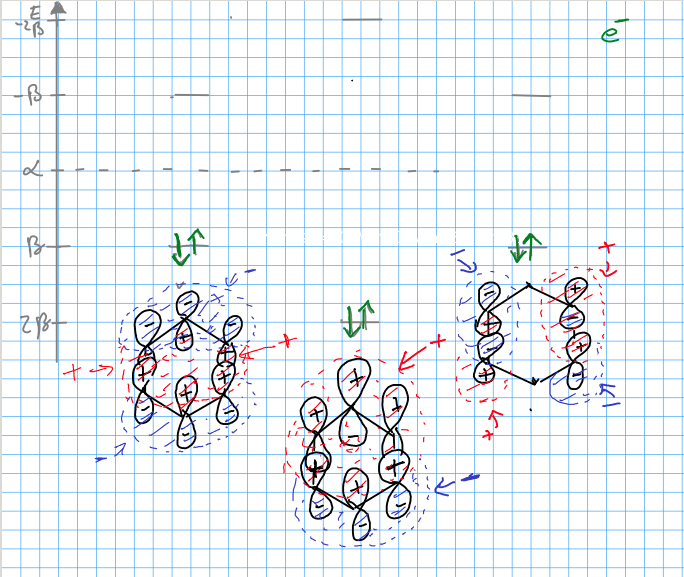
\includegraphics[width=\textwidth]{theo.png}
                \caption{Plot of energy, electron distribution and corresponding wave functions}
                \label{fig:wavef}
 \end{figure}
 
 It can easily be seen that the HOMO is $E = \beta$ and the LUMO is $E=-\beta$.

\newpage
 
\section{Computational Task: DFT calculations with Siesta}

\subsection{Geometry optimization of adenine}

\begin{table}[H]
\begin{tabular}{c|c|c|c||c|c|c|c} 
Distance in \r{A} & GGA & LDA & Exp\footnotemark[1] & Angle in degrees & GGA & LDA  & Exp\footnotemark[1]\\ 
\hline 
\hline
C2-N3 & 1.353 & 1.338 & 1.332 & N3-C4-C5 & 127.37 & 127.17 & 126.9 \\ 
\hline 
N1-C2 & 1.357 & 1.343 & 1.338 & C2-N3-C4 & 110.51 & 111.13 & 110.8 \\ 
\hline 
C6-N1 & 1.356 & 1.342 & 1.349 & N9-C4-C5 & 104.16 & 104.16 & 105.7 \\ 
\hline 
C5-C6 & 1.427 & 1.415 & 1.409 & C8-N9-C4 & 106.94 & 107.01 & 105.9 \\ 
\hline 
C4-C5 & 1.415 & 1.406 & 1.382 & N7-C8-N9 & 113.51 & 113.28 & 113.8 \\ 
\hline 
N3-C4 & 1.351 & 1.336 & 1.342 & C5-N7-C8 & 103.60 & 103.88 & 103.9 \\  
\end{tabular} 
\caption{Bond lengths and bond angles predicted by siesta and experimental data.}\label{tab:distances_and_angles}
\end{table}

\footnotetext[1]{source: Attachment1a.pdf}

With both used methods (generalized gradient approximation GGA and local density approximation LDA) the results predicted by siesta are quite close to the experimental data (table \ref{tab:distances_and_angles}). In general for the bond lengths the with LDA predicted data is quite close to the experimental results while the GGA data always overestimate the bond lengths. \\
For nearly all predicted bond angles the GGA data is closer to the experiments than the LDA data. However the LDA results vary only a litte from the GGA results.\\
So from this little trial run it seem that if one is looking for bond lengths using LDA for predictions would be a better choice than using GGA. Also the predicted angles would be pretty close to the experimental data. For more accuracy computing the bond angles GGA would possibly be an even better choice.

\newpage

\subsection{Theoretical Prediction of Watson-Crick Hydrogen-bond length in
adenine-thymine base pair}

\begin{figure}[H]
        \centering
        \begin{subfigure}[b]{0.49\textwidth}
                \centering
                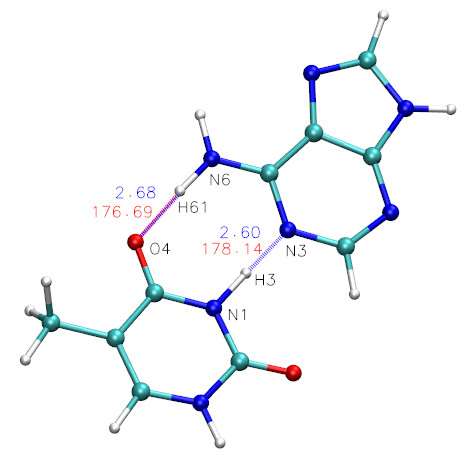
\includegraphics[width=\textwidth]{lda.jpg}
                \caption{LDA}
                \label{fig:gull}
        \end{subfigure}
        \begin{subfigure}[b]{0.49\textwidth}
                \centering
                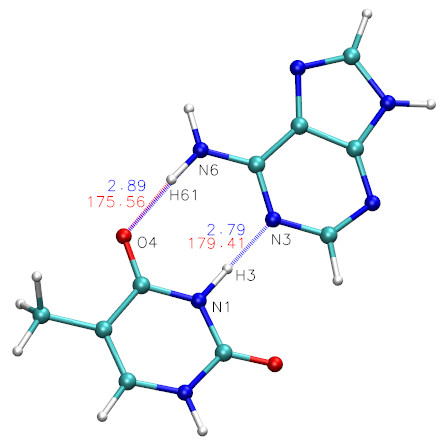
\includegraphics[width=\textwidth]{gga.jpg}
                \caption{GGA}
                \label{fig:tiger}
        \end{subfigure}
        \caption{Results for two flavours of XC functional. Blue numbers show bond lengths and red ones show bond angles.}\label{fig:ade-thy}
\end{figure}

\begin{table}[H]
\begin{tabular}{l||l|l|l}
Angle in degrees & LDA & GGA & Literature \footnotemark[2]\\ 
\hline \hline 
O4-H61-N6 & 176.7 & 175.6 & 175.8\\ 
\hline 
N1-H3-N3 & 178.1 & 179.4 & 178.1\\ 
\end{tabular}
\caption{Bond angles}\label{tab:angles}
\end{table}

\begin{table}[H]
\begin{tabular}{l||l|l|l|l}
Distance in \r{A} & LDA & GGA & Experiment 1 \footnotemark[2] & Experiment 2 \footnotemark[2] \\ 
\hline \hline 
O4-N6 & 2.68 & 2.89 & 2.95 & 2.93 \\ 
\hline 
N1-N3 & 2.60 & 2.79 & 2.82 & 2.85 \\ 
\end{tabular}
\caption{Bond lengths}\label{tab:lengths}
\end{table}

\footnotetext[2]{source: Attachment1b.pdf}

With LDA (local density approximation) and GGA (generalized gradient approximation) you get decent results. Both show that the O4-N6 bound is around $\unit[8 - 10]{\r{A}}$ longer than the N1-N3 bound. The comparison with experimental data (see table \ref{tab:lengths}) illustrates that GGA is more precise than LDA. For GGA the deviation is around $\unit[2]{\%}$ and for LDA around $\unit[10]{\%}$. However the exact error can't be specified because you don't have an isolated adenine-thymine base pair in the real world and the experimental results depend on the chemical environment.

The high precision of GGA can be explained by the fact that it uses the gradient which is non-local. In contrast LDA is a local approximation. It overestimates the bond strength regularly. Therefor the bond lengths are to short. LDA is highly precise only if you have a structure with uniform electron density.

The calculated bond angles are in conformity with calculated values that were found in Attachment1b.pdf (see Table \ref{tab:angles}). It's virtually impossible to figure out whether their calculation is more exact than ours.

For convergence GGA needed 64 steps and LDA 70 steps. A GGA step is more time consuming than a LDA step due to the use of the gradient. Therefore GGA ran for $\unit[52]{min}$ and LDA for $\unit[49]{min}$. As you can see the difference in run time is very small so that you should use GGA for all similar problems because of higher precision.

\end{document}


% =============== Comments ============
\begin{comment}
\verb{x_init {}}

\begin{figure}[H]
	\resizebox{1\textwidth}{!{\input{../plots/NAME.pgf}}
	\caption{CAPTION}\label{fig:NAME}
\end{figure}
\end{comment}
